\section{Theorie}
\label{sec:Theorie}

Die Aussage des Dulong-Petitschen-Gesetzt ist
\begin{equation}
    C_\text{V} = \left ( \frac{\symup{dQ}}{\symup{dT}} \right )_\text{V} = \left ( \frac{\symup{dU}}{\symup{dT}} \right )_\text{V}  .
    \label{eqn:dulong}
\end{equation}
$Q$ stellt dabei eine Wärmemenge, $T$ eine Temperatur und $U$ die innere Energie eines Mol eines Stoffes da.
$C_\text{V}$ ist die molare Wärmekapazität bei konstantem Volumen.

Weiterhin geht aus \eqref{eqn:dulong} hervor, dass
\begin{equation}
    C_\text{V} = 3R
    \label{eqn:dulong_klassisch}
\end{equation}
ist. Hierbei stellt $R$ die Allgemeine Gaskonstante da.
Es ist technisch schwierig $C_\text{V}$ zu messen, deswegen wird ebenfalls die Gleichung
\begin{equation}
    C_\text{V} = C_\text{p} - 9 \alpha^2 \kappa V_0 T
    \label{eqn:kapa_mol}
\end{equation}
eingeführt.
Diese stellt die molare Wärmekapazität bei gleich bleibenem Druck und gleich bleibenem Volumen in Zusammenhang.
$\kappa$ stellt hier das Kompressionsmodul, $\alpha$ den Ausdehnungskoeffizienten und $V_0$ das Molvolumen da.
Zur Vereinfachung der Auswertung wird Gleichung \eqref{eqn:kapa_mol} noch umgeschrieben in
\begin{equation}
    C_\text{V} = c_\text{k} M - 9\alpha^2 \kappa \frac{M}{\rho}T.
\end{equation}
$c_\text{k}$ steht für die spezifische Wärmekapazität, $M$ für die molare Masse und $\rho$ für die Dichte.
Das klassische System betrachtet die Kräfte zwischen Atomen in Festkörpern als Federn.
Ihre Kraft kann durch das Hook'sche Gesetzt bestimmt werden.
Daraus folgt, dass ein Atom pro Bewegungsfreiheitsgrad eine gesamte innere Energie von
\begin{equation*}
    \left < U \right > = kT
\end{equation*}
hat.
Für alle Freiheitsgrade eines Atoms ist die gesamte innere Energie also
\begin{equation*}
    \left < U \right > = 3RT.
\end{equation*}
Laut der Quantenmechanik, kann Energie nur in gequantelten Teilen abgegeben werden.
Dies steht in Widerspruch mit der klassischen Physik.
Für hohe Temperaturen ist jedoch trotzdem zu beobachten, dass 
\begin{equation*}
    C_\text{V} \approx 3 R
\end{equation*}
gilt.
Hier decken sich also die quantenmechanische Beschreibung und die klassische.
Die meisten Stoffe erreichen diesen Punkt schon bei Zimmertemperatur, einige aber erst bei höheren Temperaturen.

Um nun die spezifische Wärmekapazität einer Probe zu bestimmen wird
\begin{equation}
   c_\text{k} = \frac{(c_\text{w}m_\text{w} + c_\text{g}m_\text{g})(T_\text{m}-T_\text{w})}{m_\text{k}(T_\text{k}-T_\text{m})} 
   \label{eqn:kapa}
\end{equation}
genutzt.
Für $c_\text{w}$ wird die spezifische Wärmekapazität von Wasser eingesetz und für $m_\text{w}$ wird die Masse des genutzten Wassers eingesetzt.
Die Wärmekapazität $c_\text{g}m_\text{g}$ wird während des Versuchs bestimmt.
$T_\text{m}$ ist die Mischtemperatur, welche sich nach einiger Zeit im Dewar-Gefäß einstellt.
$T_\text{w}$ ist die Temperatur des Wasser im Dewar-Gefäß bevor die Probe hinein gegeben wurde.
$m_\text{k}$ und $T_\text{k}$ bezeichnen die Masse der Probe und die Temperatur der Probe bevor diese in das Dewar-Gefäß gegeben wird.

Zur Bestimmung der Wärmekapazität des Dewar-Gefäß werden zwei Wassermengen genutzt.
Die Masse dieser Wassermengen wird $m_\text{x}$ und $m_\text{y}$ genannt.
Die beiden Wassermengen, die genutzt werden haben die Temperatur $T_\text{x}$ und $T_\text{y}$.
$T_\text{m}$ ist hier, wie oben, die Mischtemperatur die sich nach einiger Zeit im Dewar-Gefäß einstellt.
Nun kann mit der Formel
\begin{equation}
    c_\text{g} m_\text{g} = \, \frac{c_\text{w}m_\text{y}(T_\text{y}-T_\text{m})-c_\text{w}m_\text{x}(T_\text{m}-T_\text{x})}{T_\text{m}-T_\text{x}}
    \label{eqn:dewar}
\end{equation}
die Wärmekapazität des Dewar-Gefäß bestimmt werden.
Für die Auswertung werden einige Materialeigenschaften benötigt, diese sind in der Tabelle \ref{fig:material} zu finden.
\begin{figure}
    \centering
    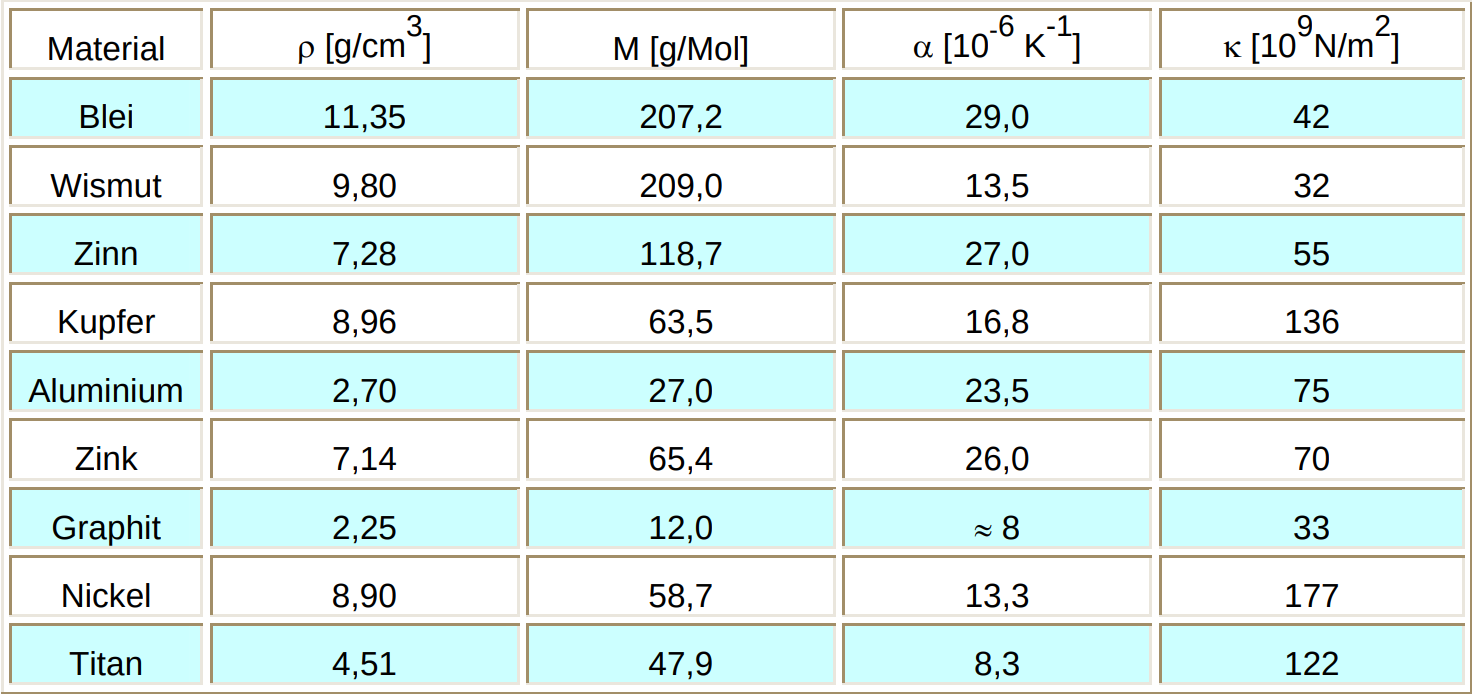
\includegraphics[width=\textwidth]{content/data/tabelleV201.png}
    \caption{Physikalische Eigenschaften einiger Materiale, entnommen aus \cite{anleitung}.}
    \label{fig:material}
\end{figure}